\documentclass[tikz,border=.5cm]{standalone}
\begin{document}
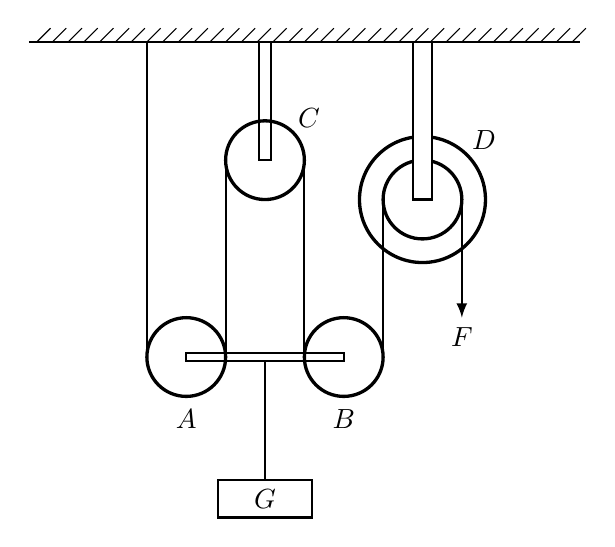
\begin{tikzpicture}
    \draw[thick] (-4,0) -- (3,0);
    \foreach \x in {-3.9,-3.7,...,2.9} {
        \draw[shift={(\x,0)},black] (0pt,0pt) -- (5pt,5pt);
    }
    \draw[very thick] 
        (-2,-4) circle[radius=.5] node[below=15pt] {$A$}
        (0,-4) circle[radius=.5] node[below=15pt] {$B$}
        (-1,-1.5) circle[radius=.5] node[above right=8pt] {$C$}
        (1,-2) circle[radius=.5] circle[radius=.8] node[above right=14pt] {$D$}
        ;
    \draw[thick] 
    (-1-0.08,-1.5) rectangle (-1+0.08,0)
    (-2,-4-0.05) rectangle (0,-4+0.05);
    \filldraw[fill=white,thick] 
    (1-0.12,-2) rectangle (1+0.12,0);
    \draw[thick] (-1,-4-0.05) -- ++(0,-1.5) 
                 node[anchor=north,rectangle,draw,minimum width=1.2cm] {$G$};
    \draw[-latex,xshift=-0.5cm,thick] 
        (-2,0) -- ++(0,-4) 
        ++(1,0) -- ++(0,2.5)
        ++(1,0) -- ++(0,-2.5)
        ++(1,0) -- ++(0,2)
        ++(1,0) -- ++(0,-1.5) node[below] {$F$}
        ;
\end{tikzpicture}

\end{document}